\pagestyle{headings}
\section{Introdução}
A Visão Computacional é uma área de pesquisa que se ocupa em utilizar imagens em 2D de um cenário, obtidas de uma ou mais câmeras digitais para produzir uma construção virtual em 3D, ou extrair qualquer outro tipo de informação útil como localização e transferência de pontos de uma imagem para outra. A captação da geometria 3D de um cenário a partir de imagens produzidas por câmeras, analisando a disparidade entre elementos correspondentes nessas imagens é chamada de visão {\it estereoscópica}, da qual a visão computacional se utiliza para desenvolver modelos adequados à descrição geométrica tanto da cena em questão como das câmeras que fazem a projeção da cena na imagem 2D.  

\begin{figure}[!htb]
\centering
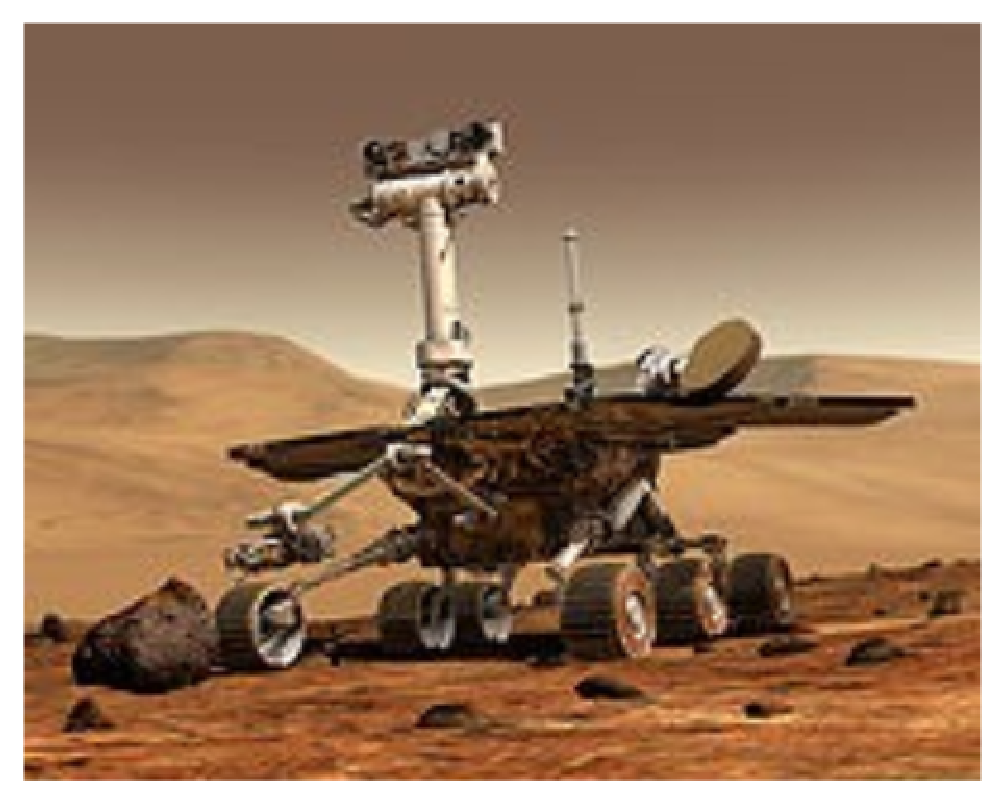
\includegraphics[scale=.5]{mars-rover}
\caption{{\it O maior passo no uso de visão computacional em pesquisas interplanetárias foi dado na missao NASA/JPL Mars Exploration Rover (MER).}}
\label{fig.mars-rover}
\end{figure}

A Geometria Projetiva é a principal teoria matemática usada em visão computacional. Com a introdução de algumas definições e conceitos, a geometria projetiva pode ser estudada em termos de Álgebra Linear, onde tal abordagem traz alguns benefícios e é amplamente utilizada por pesquisadores dessa área, mas também possui algumas limitações. Em pesquisas mais recentes, verificou-se a eficácia do uso de técnicas de Geometria Algébrica em resoluções de sistemas de equações polinomiais, oriundos de problemas de visão computacional. Mais recentemente ainda, \citep{tese-fabbri} introduziram uma abordagem em termos de Geometria Diferencial, onde é possível aplicar o Cálculo Diferencial trabalhando diretamente com as equações algébricas.


\subsection*{Motivação}
As motivações para a pesquisa estão ligadas à atualidade do tema e consequentemente suas aplicações em diversas áreas. A extração de informação da geometria 3D de um ambiente pode, por exemplo, ser utilizada na determinação da orientação e posição de veículos autônomos, para que o mesmo identifique a trajetória para o seu objetivo considerando a possibilidade de obstáculos. Um exemplo famoso, segundo \citep{mars-rover}, é a aplicação em pesquisas interplanetárias onde foram usados algoritmos de visão computacional em veículos de exploração de Marte (Mars Exploration Rover - MER, em inglês), observado na figura \ref{fig.mars-rover}.


Uma aplicação mais recente foi a reconstrução virtual de objetos, estátuas ou monumentos de valor histórico e cultural que tenham sido destruídos pela ação do tempo ou do homem (possivelmente em guerras), através da aquisição de imagens em acervos ou na internet. Um exemplo é o Museu de Mosul {\footnote{Outros exemplos podem ser encontrados em http://www.projectmosul.org/}}, no Iraque, atacado pelo 
Estado Islâmico em 2015, que teve algumas de suas obras reconstruídas como podemos visualizar na figura \ref{fig.mossul}.

\begin{figure}[!htb]
\centering
\subfloat{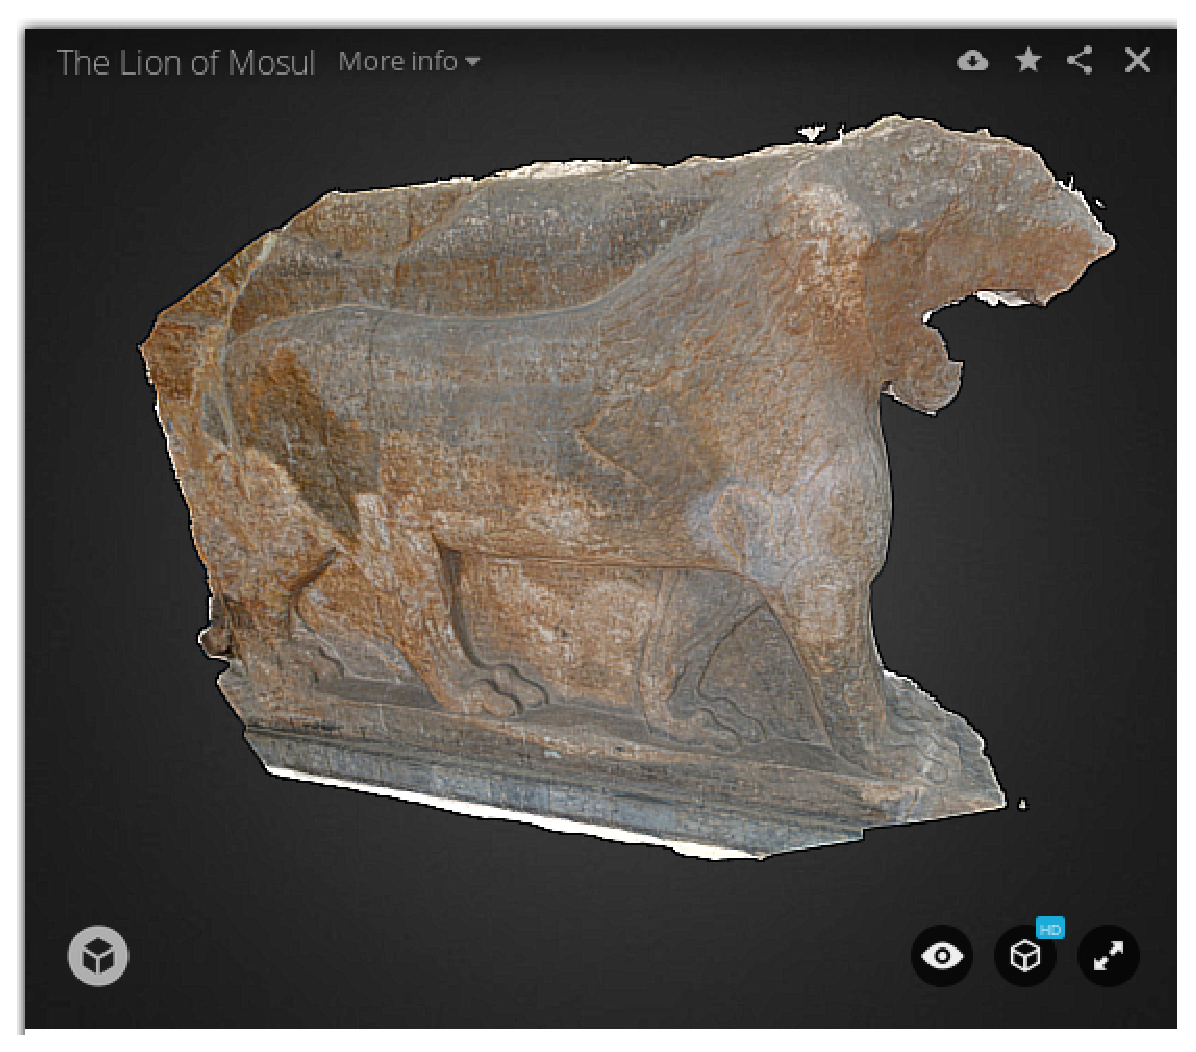
\includegraphics[scale=.35]{leao-mosul}}
\quad
\subfloat{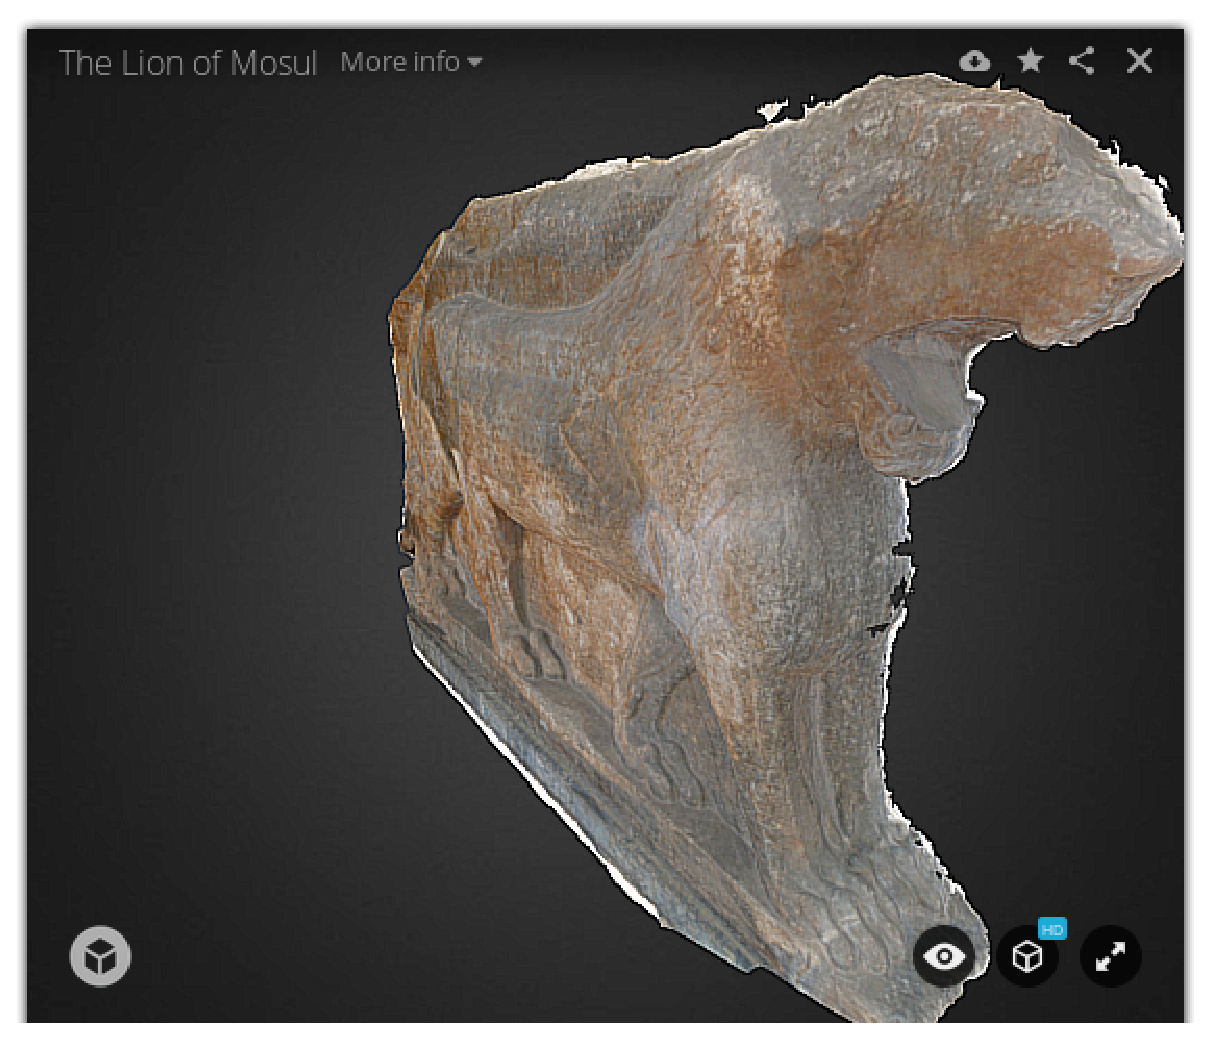
\includegraphics[scale=.35]{lion-mosul-2}}
\caption{{\it A reconstrução do Leão de Mosul, um dos artefatos destruídos por extremistas religiosos em 2015 no Iraque.}}
\label{fig.mossul}
\end{figure}

As aplicações de visão computacional são bastante variadas, com pesquisas em outras áreas como astronomia, medicina e química. Para se ter uma ideia, \citep{ballard-82} já apresentavam imagens e tabelas com resumos de aplicações em oito áreas diferentes no início dos anos 1980.  

Novos avanços em reconstrução 3D vêm sendo realizados constantemente como observamos em \citep{fabbri-drawing}, que apresentam uma abordagem para a reconstrução de um esboço 3D (3D drawing em inglês) de uma cena. Isto é, um conjunto de fragmentos de curvas em 3D interligadas de forma que preserve suas relações espaciais, capturadas em forma de gráficos a partir de um grande conjunto de dados de multivisão. A ideia base é aprimorar uma abordagem anterior (3D curve sketch) divulgada pelos mesmos autores, \citep{fabbri-sketch}, conforme exemplo visualizado na figura \ref{fig.drawing}.
\begin{figure}[!htb]
\centering
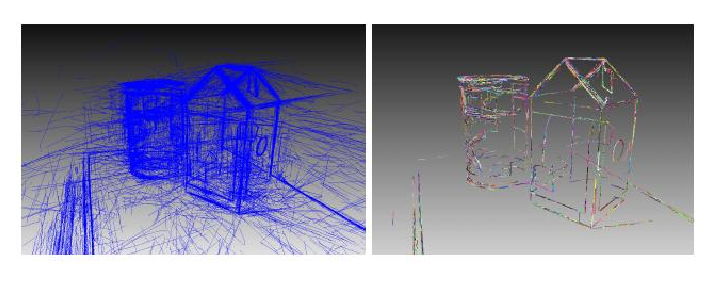
\includegraphics[scale=1.1]{3D-drawing}
\caption{{\it Uma comparação visual: à esquerda os resultados com o 3D curve sketch e à direita os resultados após o aprimoramento com 3D drawing. Repare na redução significante de outliers sem prejuízo do esboço da superfície.}}
\label{fig.drawing}
\end{figure}

A maioria dos métodos de reconstrução não utilizam geometria diferencial de curvas, mas se baseiam em correlacionar pontos de interesse através das imagens e produzem uma desorganizada nuvem de pontos em 3D, figura \ref{fig.medusa}. Tais métodos obtêm sucesso em ambientes controlados, com cenas em larga escala e imagens ricas em textura, mas não podem ser aplicados em configurações gerais. Não podem reconstruir superfícies suaves e homogêneas nem suas fronteiras devido a esparsidade de pontos de interesse, como também não podem reconstruir regiões que se alteram drasticamente com a mudança de luz ambiente. Exemplos de imagens sujeitas a essas limitações são dados na figura \ref{fig.carro-objeto-curvo}.
\begin{figure}[!htb]
\centering
\subfloat{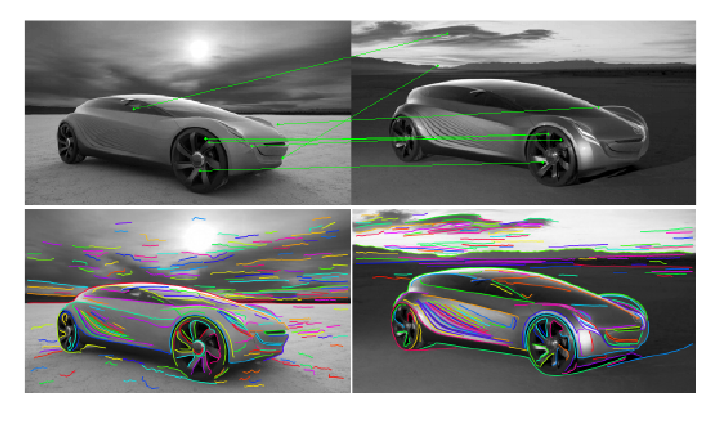
\includegraphics[scale=.76]{carro}}
\quad
\subfloat{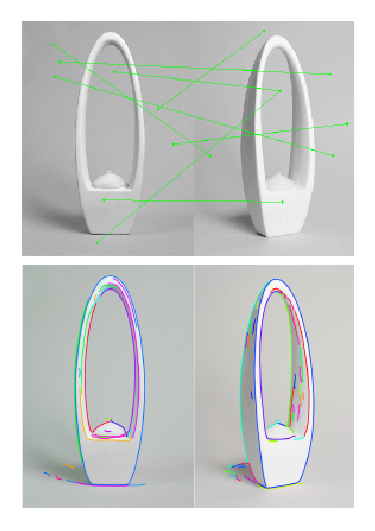
\includegraphics[scale=.6]{objeto-curvo}}
\caption{{\it Exemplos de objetos que não podem ser reconstruídos através da abordagem tradicional usando pontos de interesse e a geometria epipolar.}}
\label{fig.carro-objeto-curvo}
\end{figure}  
Daí são utilizadas outras técnicas de melhoramento dos resultados, como a Interpolação de Pontos e Texturização, mas que não fornecem um resultado plenamente satisfatório. Podemos ver as fases desse processo em um exemplo no conjunto de imagens na figura\ref{fig.medusa}.

Portanto, ainda é necessário que se continuem as pesquisas em visão computacional, e o presente trabalho tem a finalidade de, primeiramente, detalhar as abordagens de artigos recentes na busca de novas combinações de ferramentas matemáticas que possam melhorar as atuais abordagens e atenuar o esforço computacional. Segundo, a verificação dos benefícios obtidos com o uso da geometria trifocal em transferência de pontos e reconstrução 3D em comparação com a geometria epipolar (mais usada atualmente), tudo com o objetivo de auxiliar na construção de uma nova abordagem usando geometria diferencial trifocal.

\begin{figure}[!htb]
\centering
\subfloat{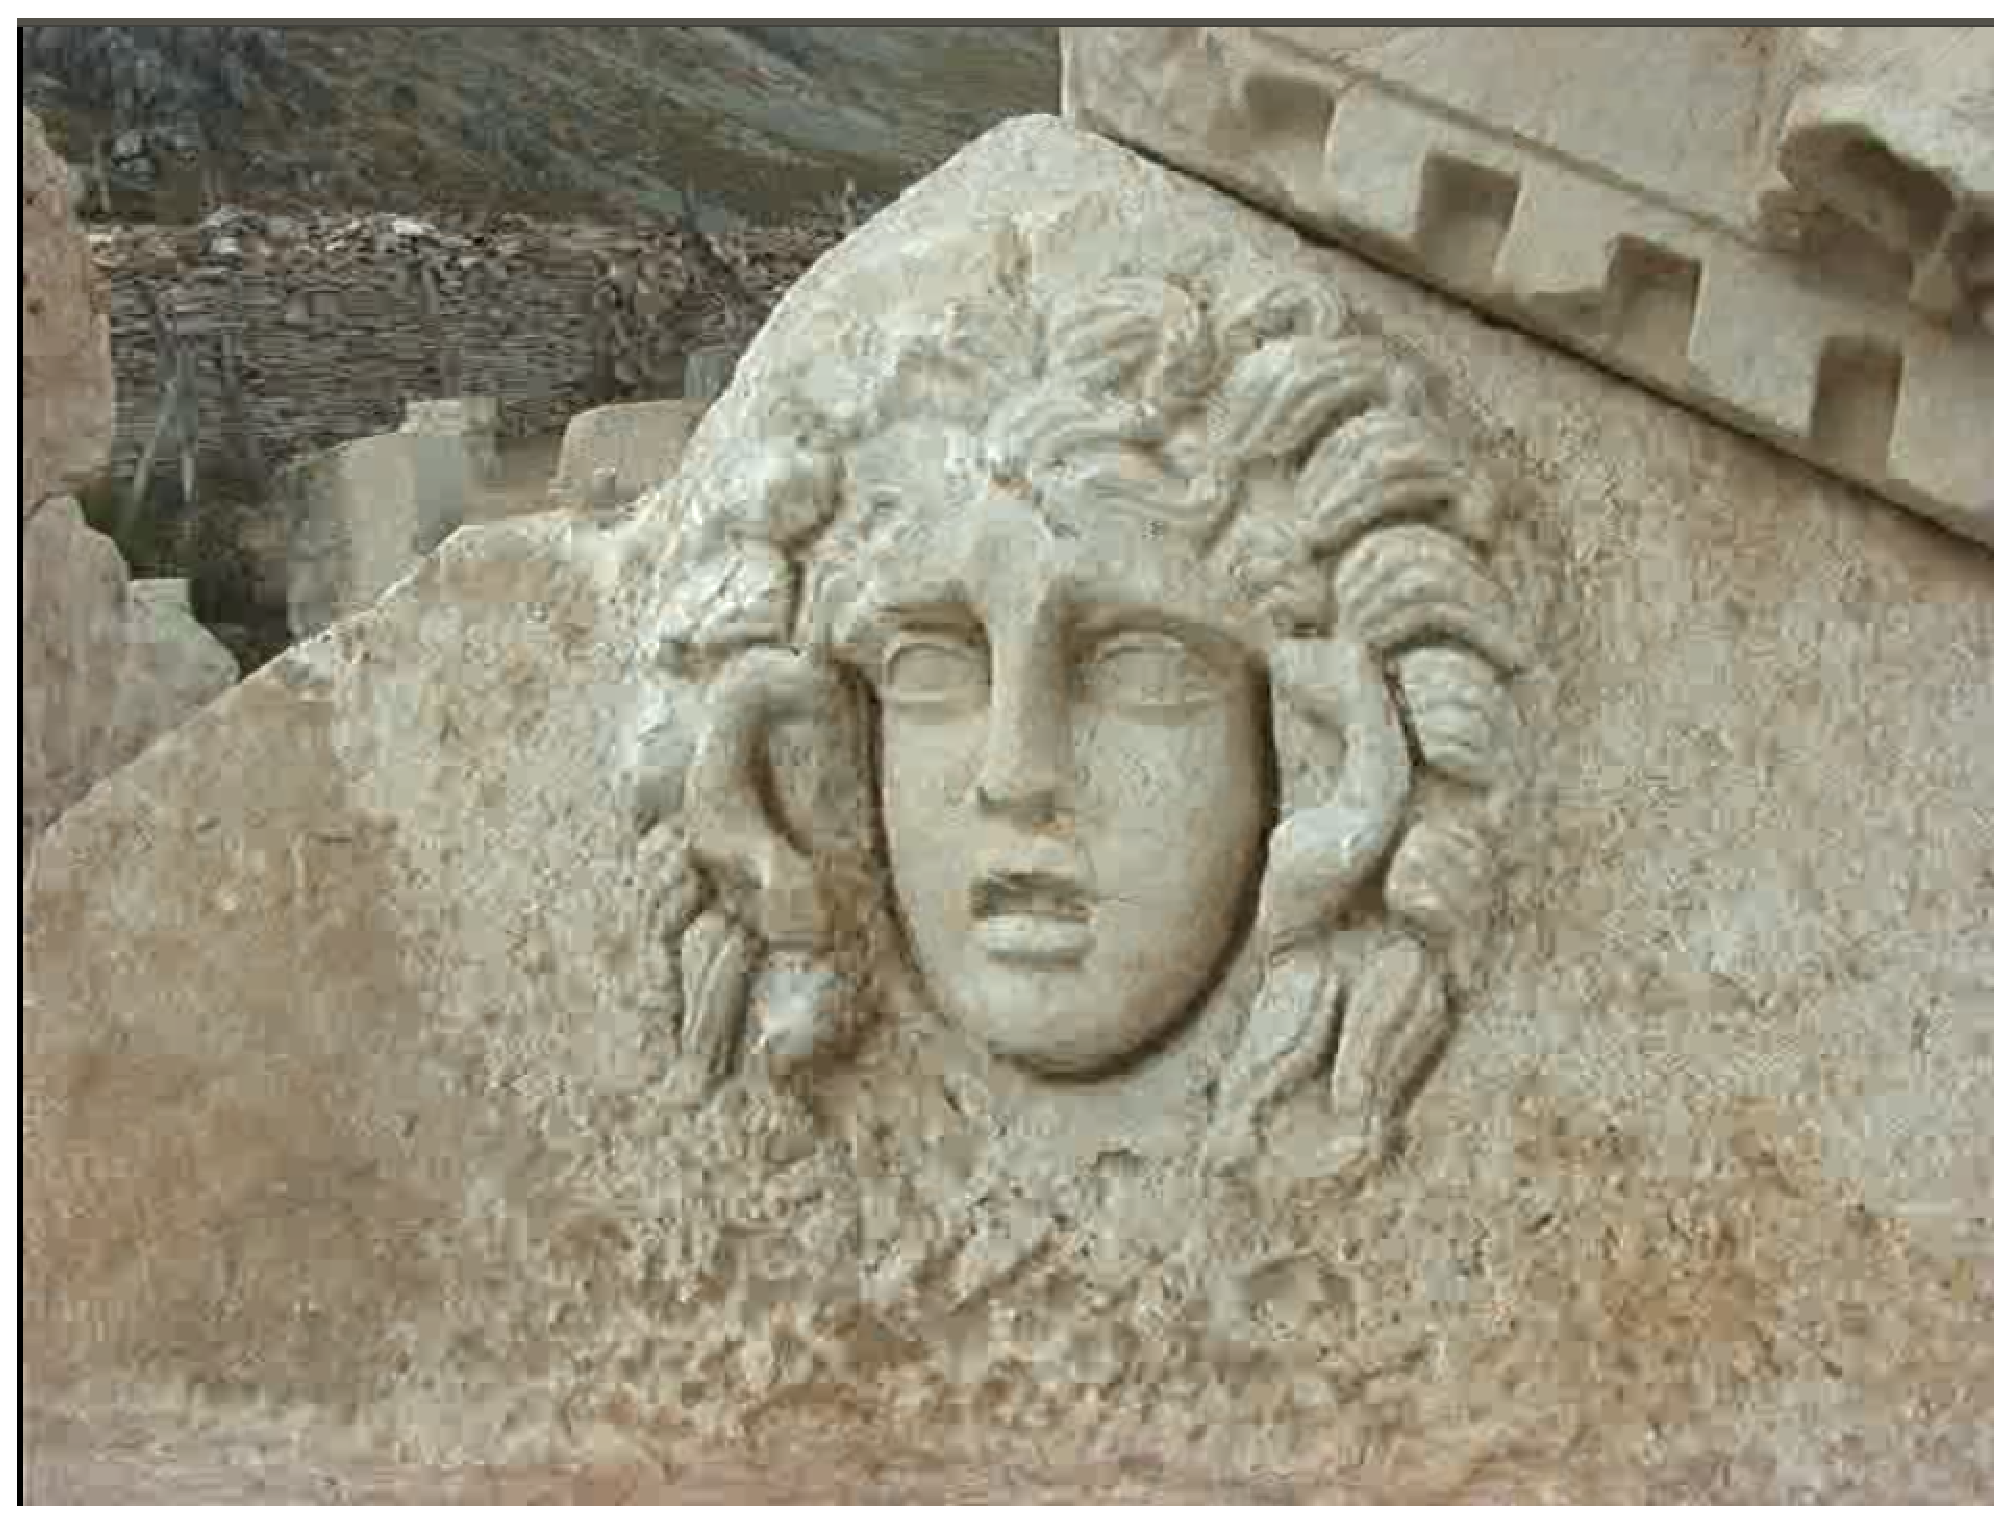
\includegraphics[scale=.2]{medusa1}}
\quad
\subfloat{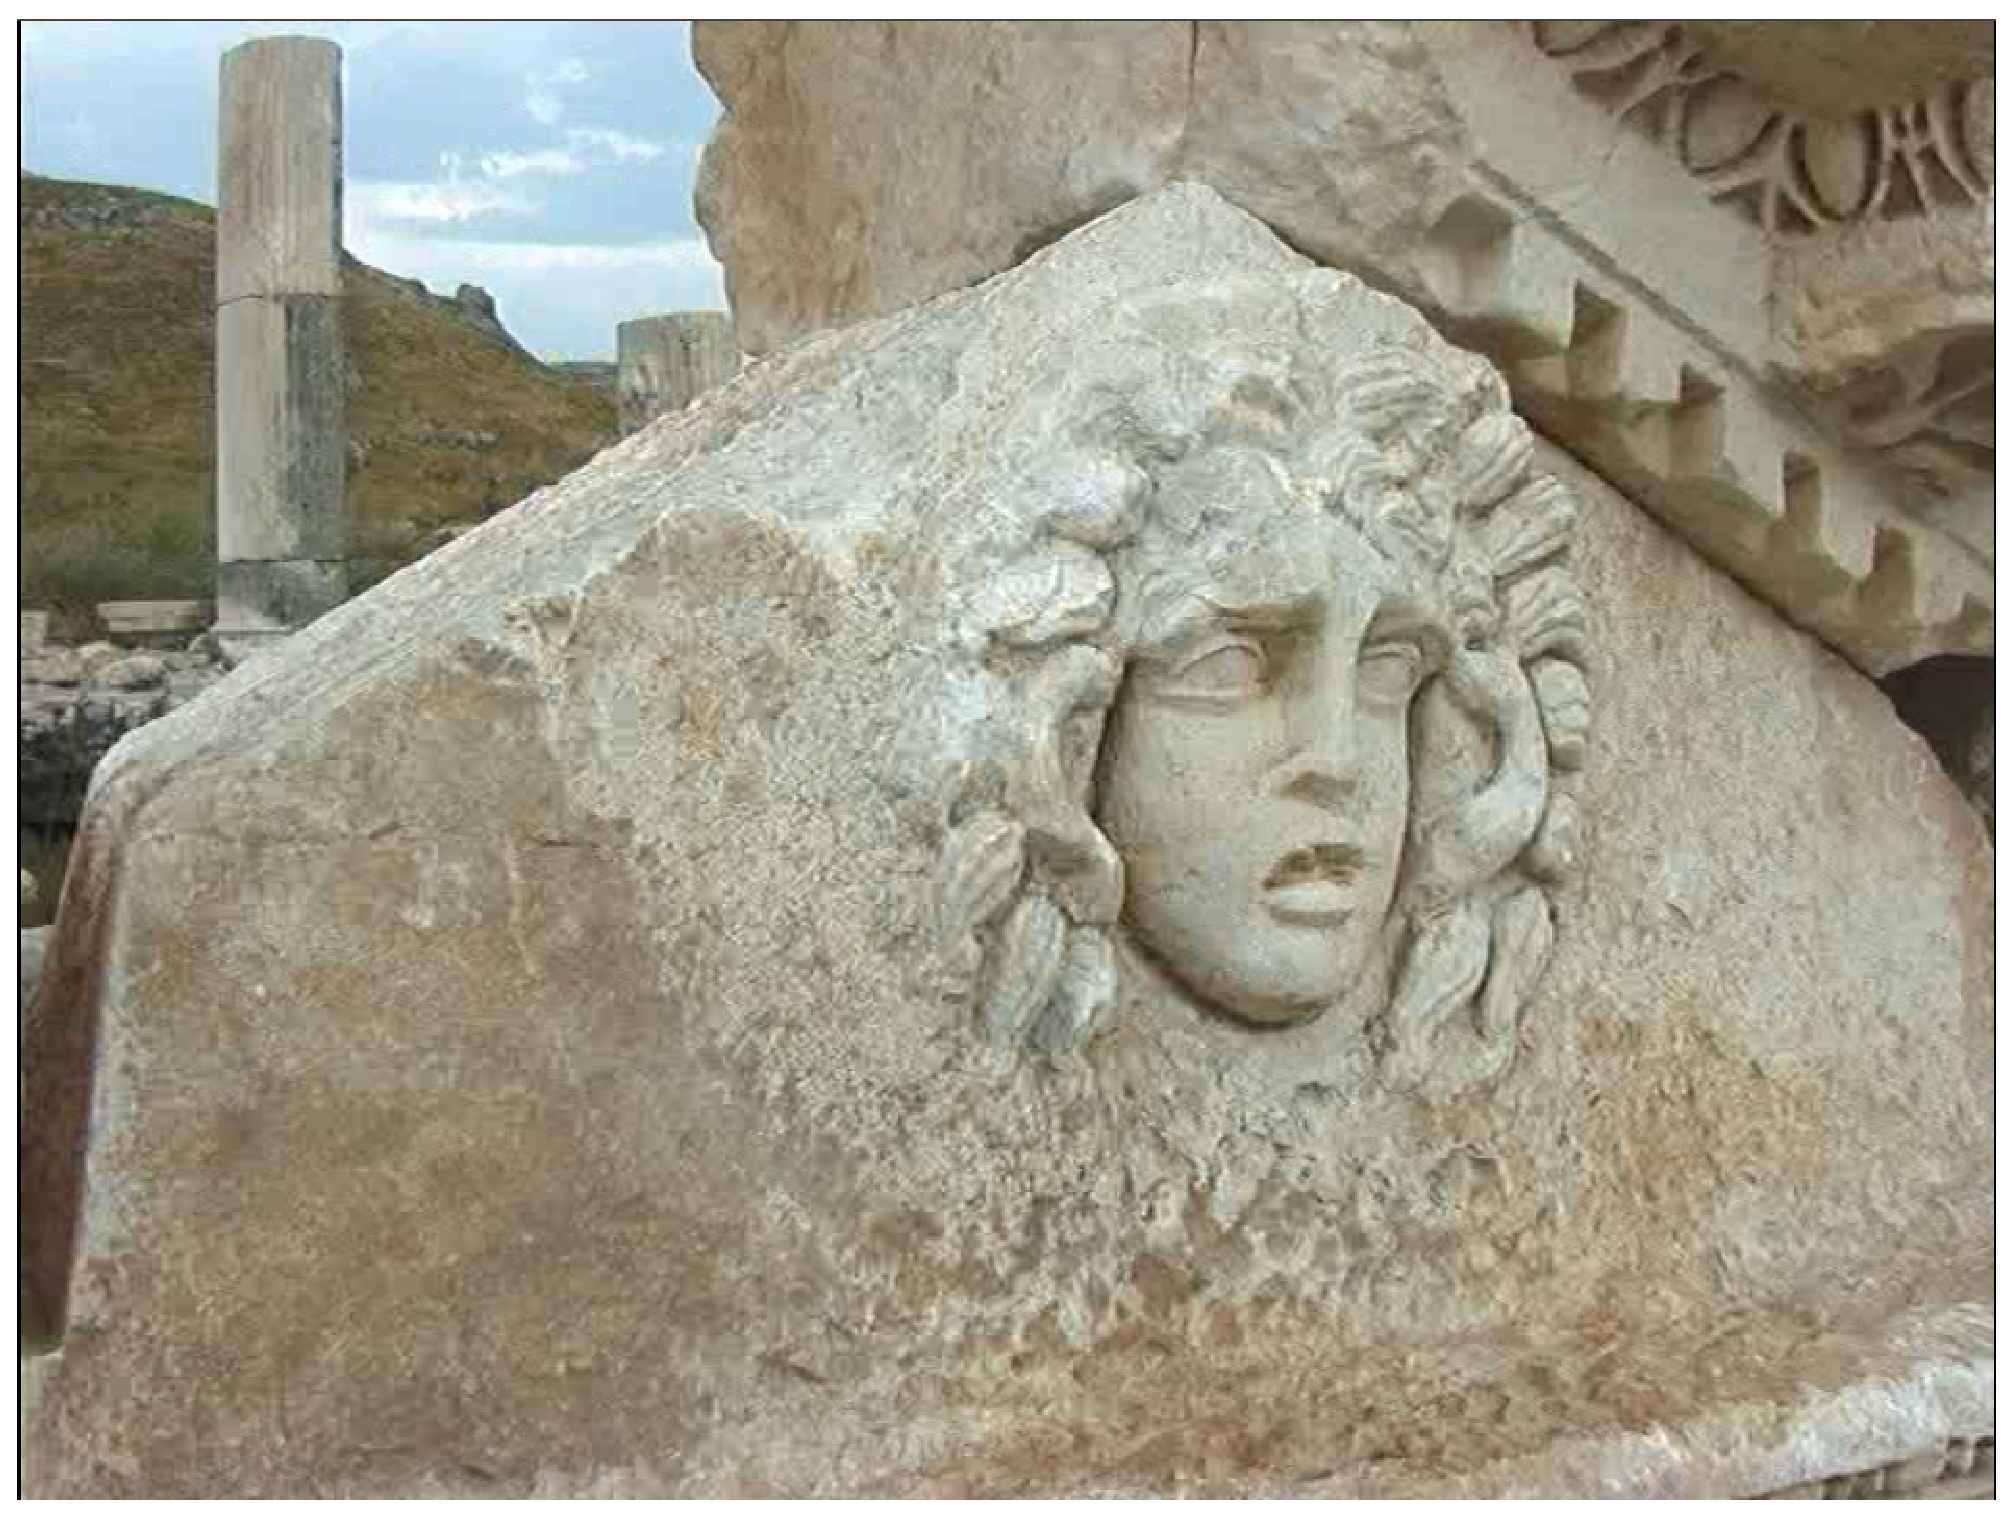
\includegraphics[scale=.2]{medusa2}}
\\
\subfloat{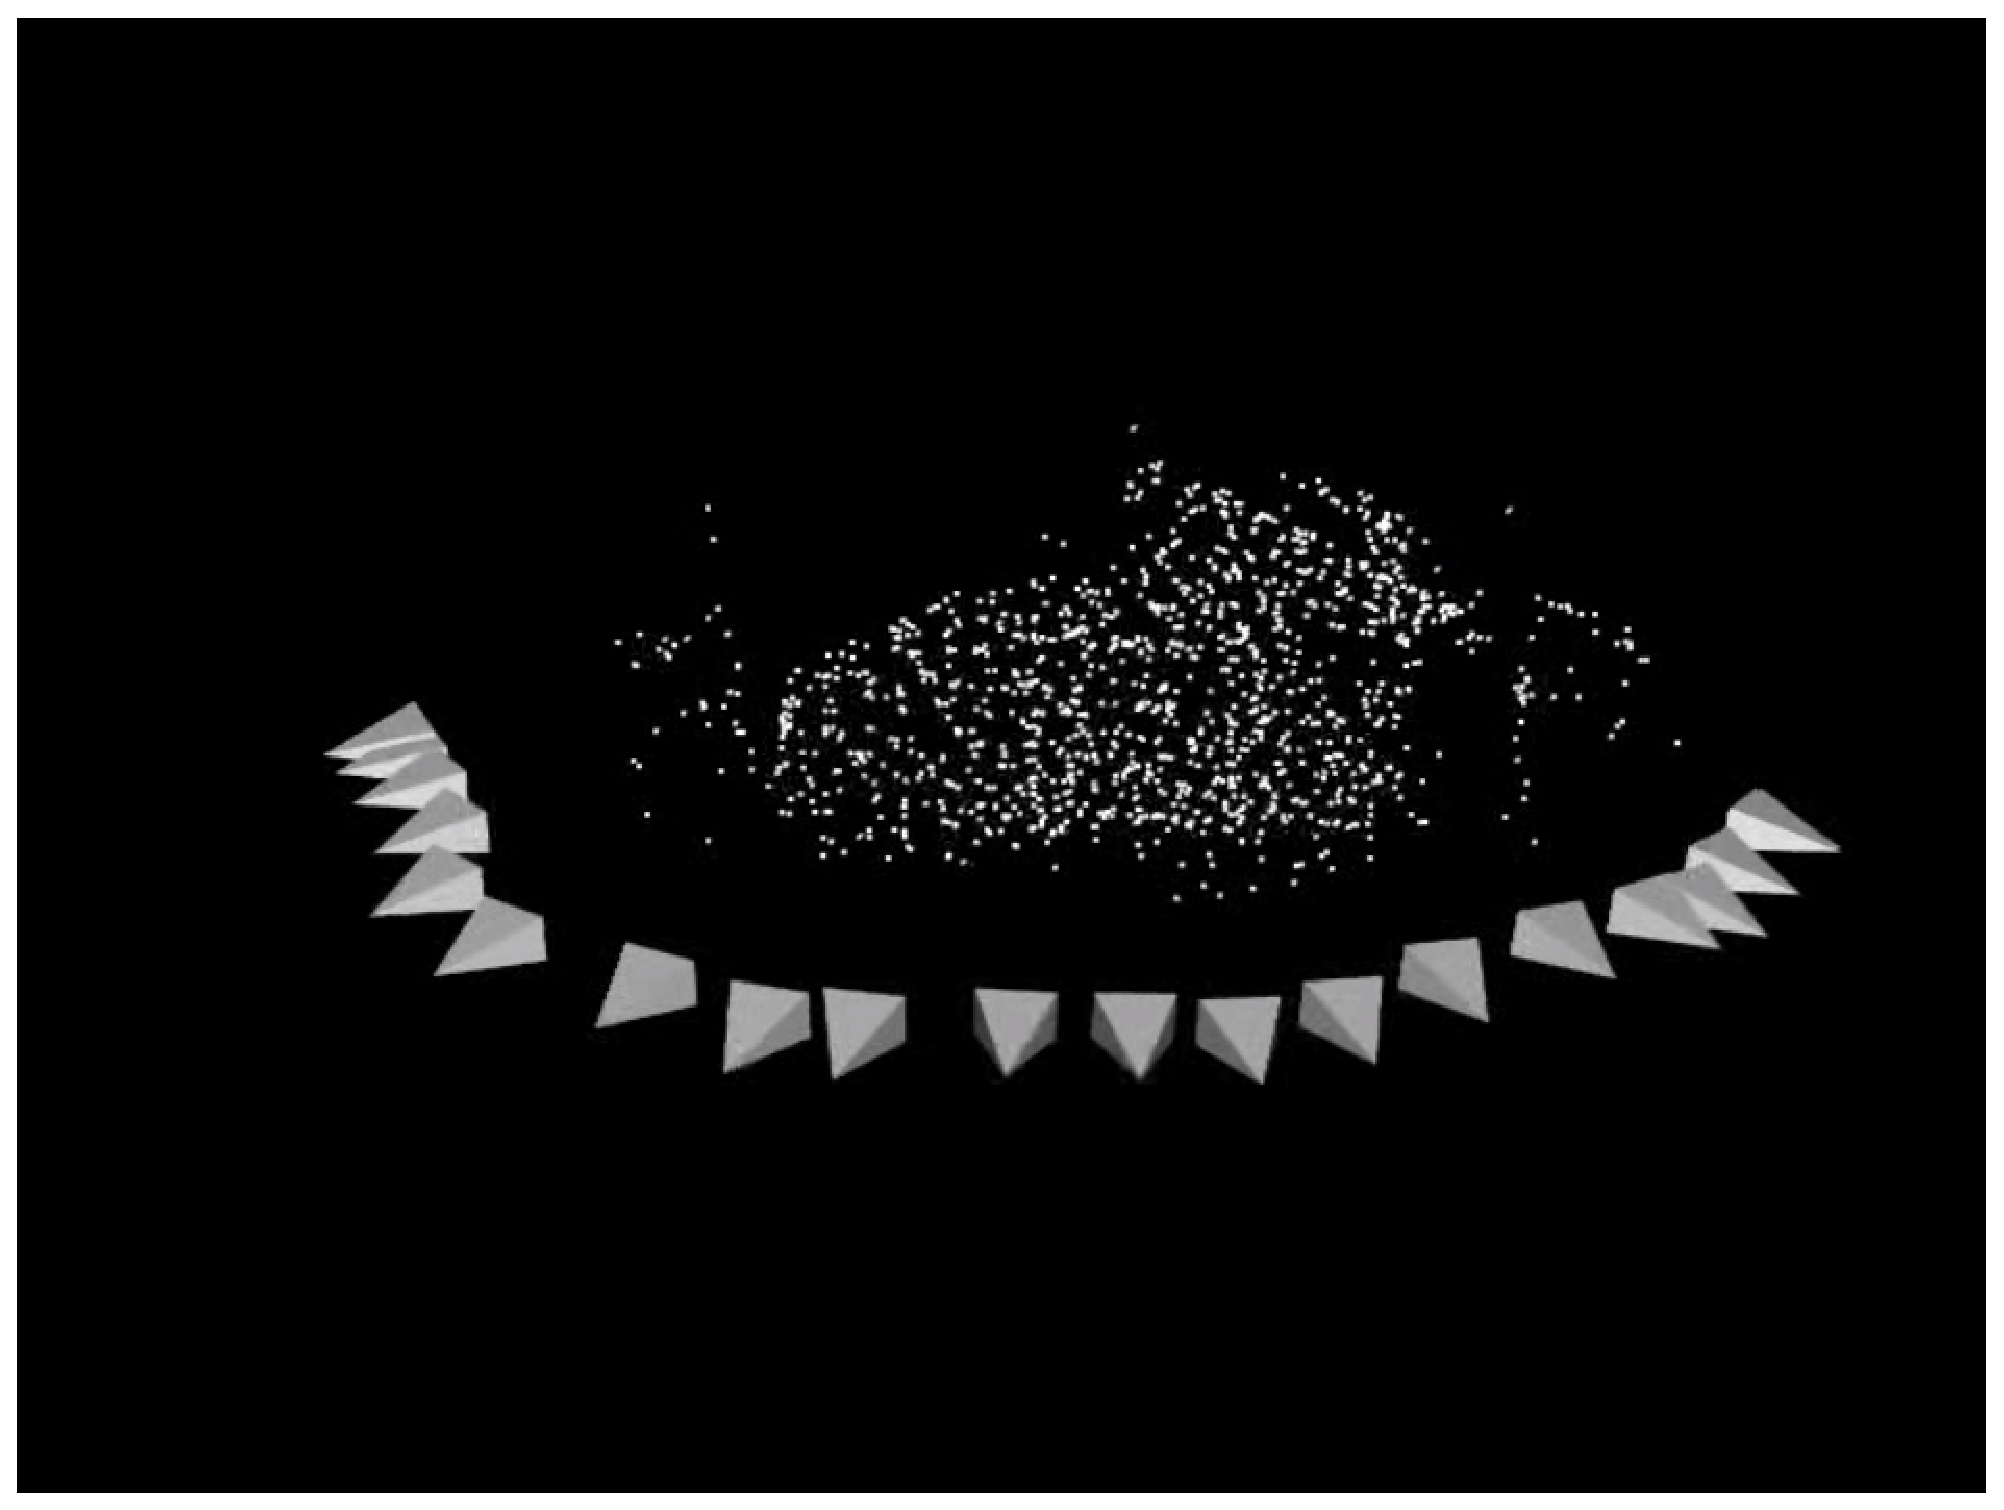
\includegraphics[scale=.2]{nuvem1}}
\quad
\subfloat{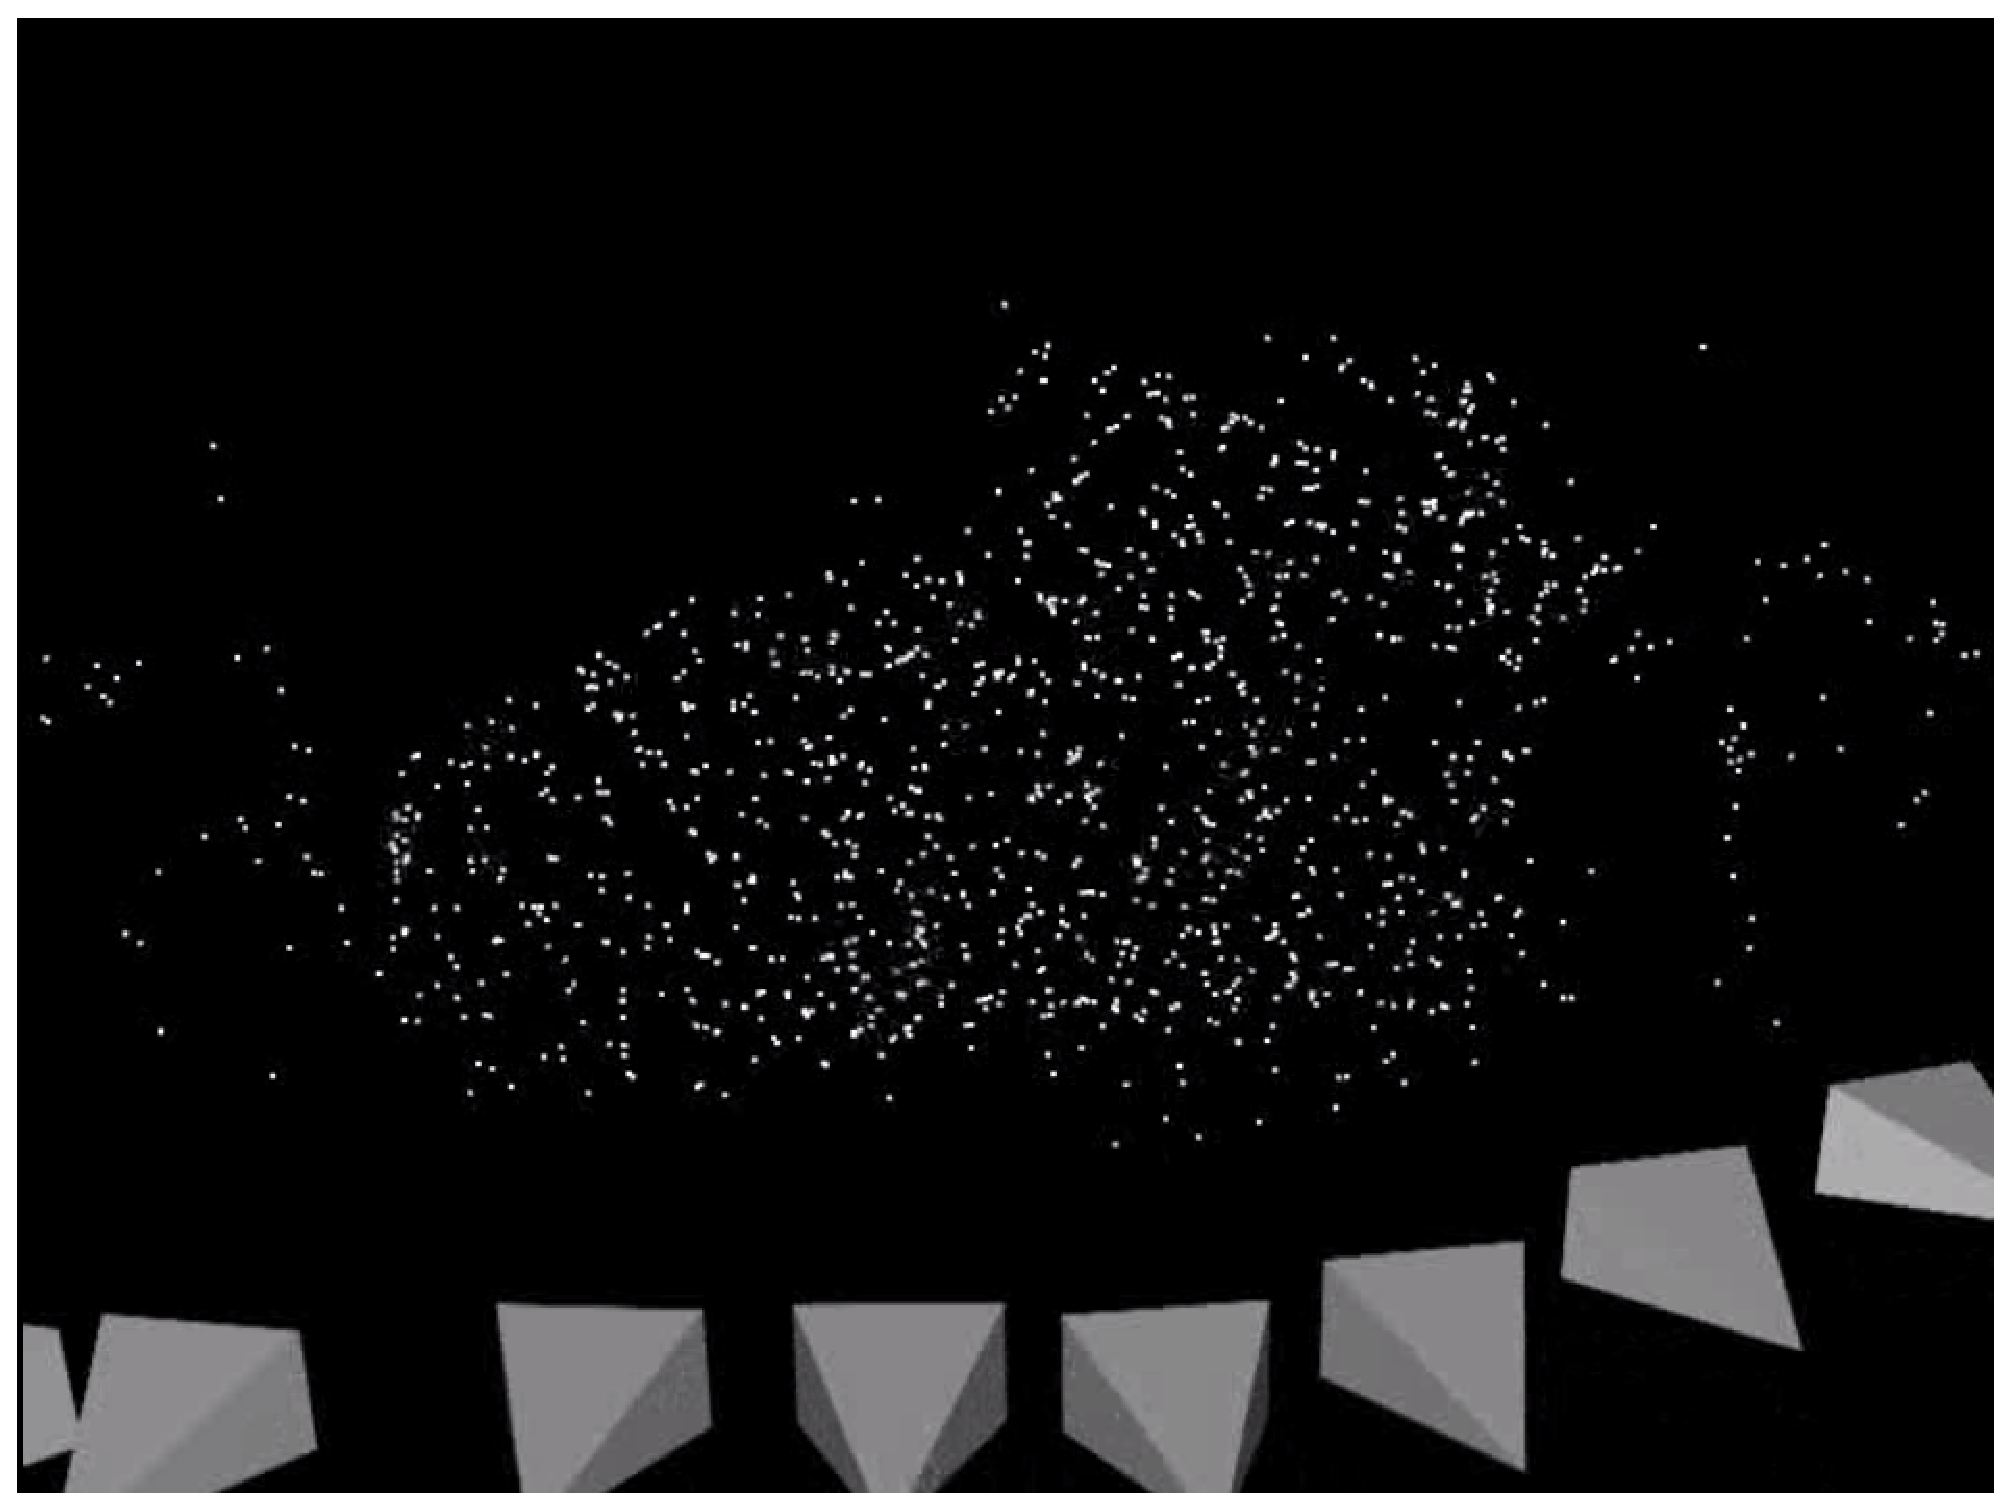
\includegraphics[scale=.2]{nuvem2}}
\\
\subfloat{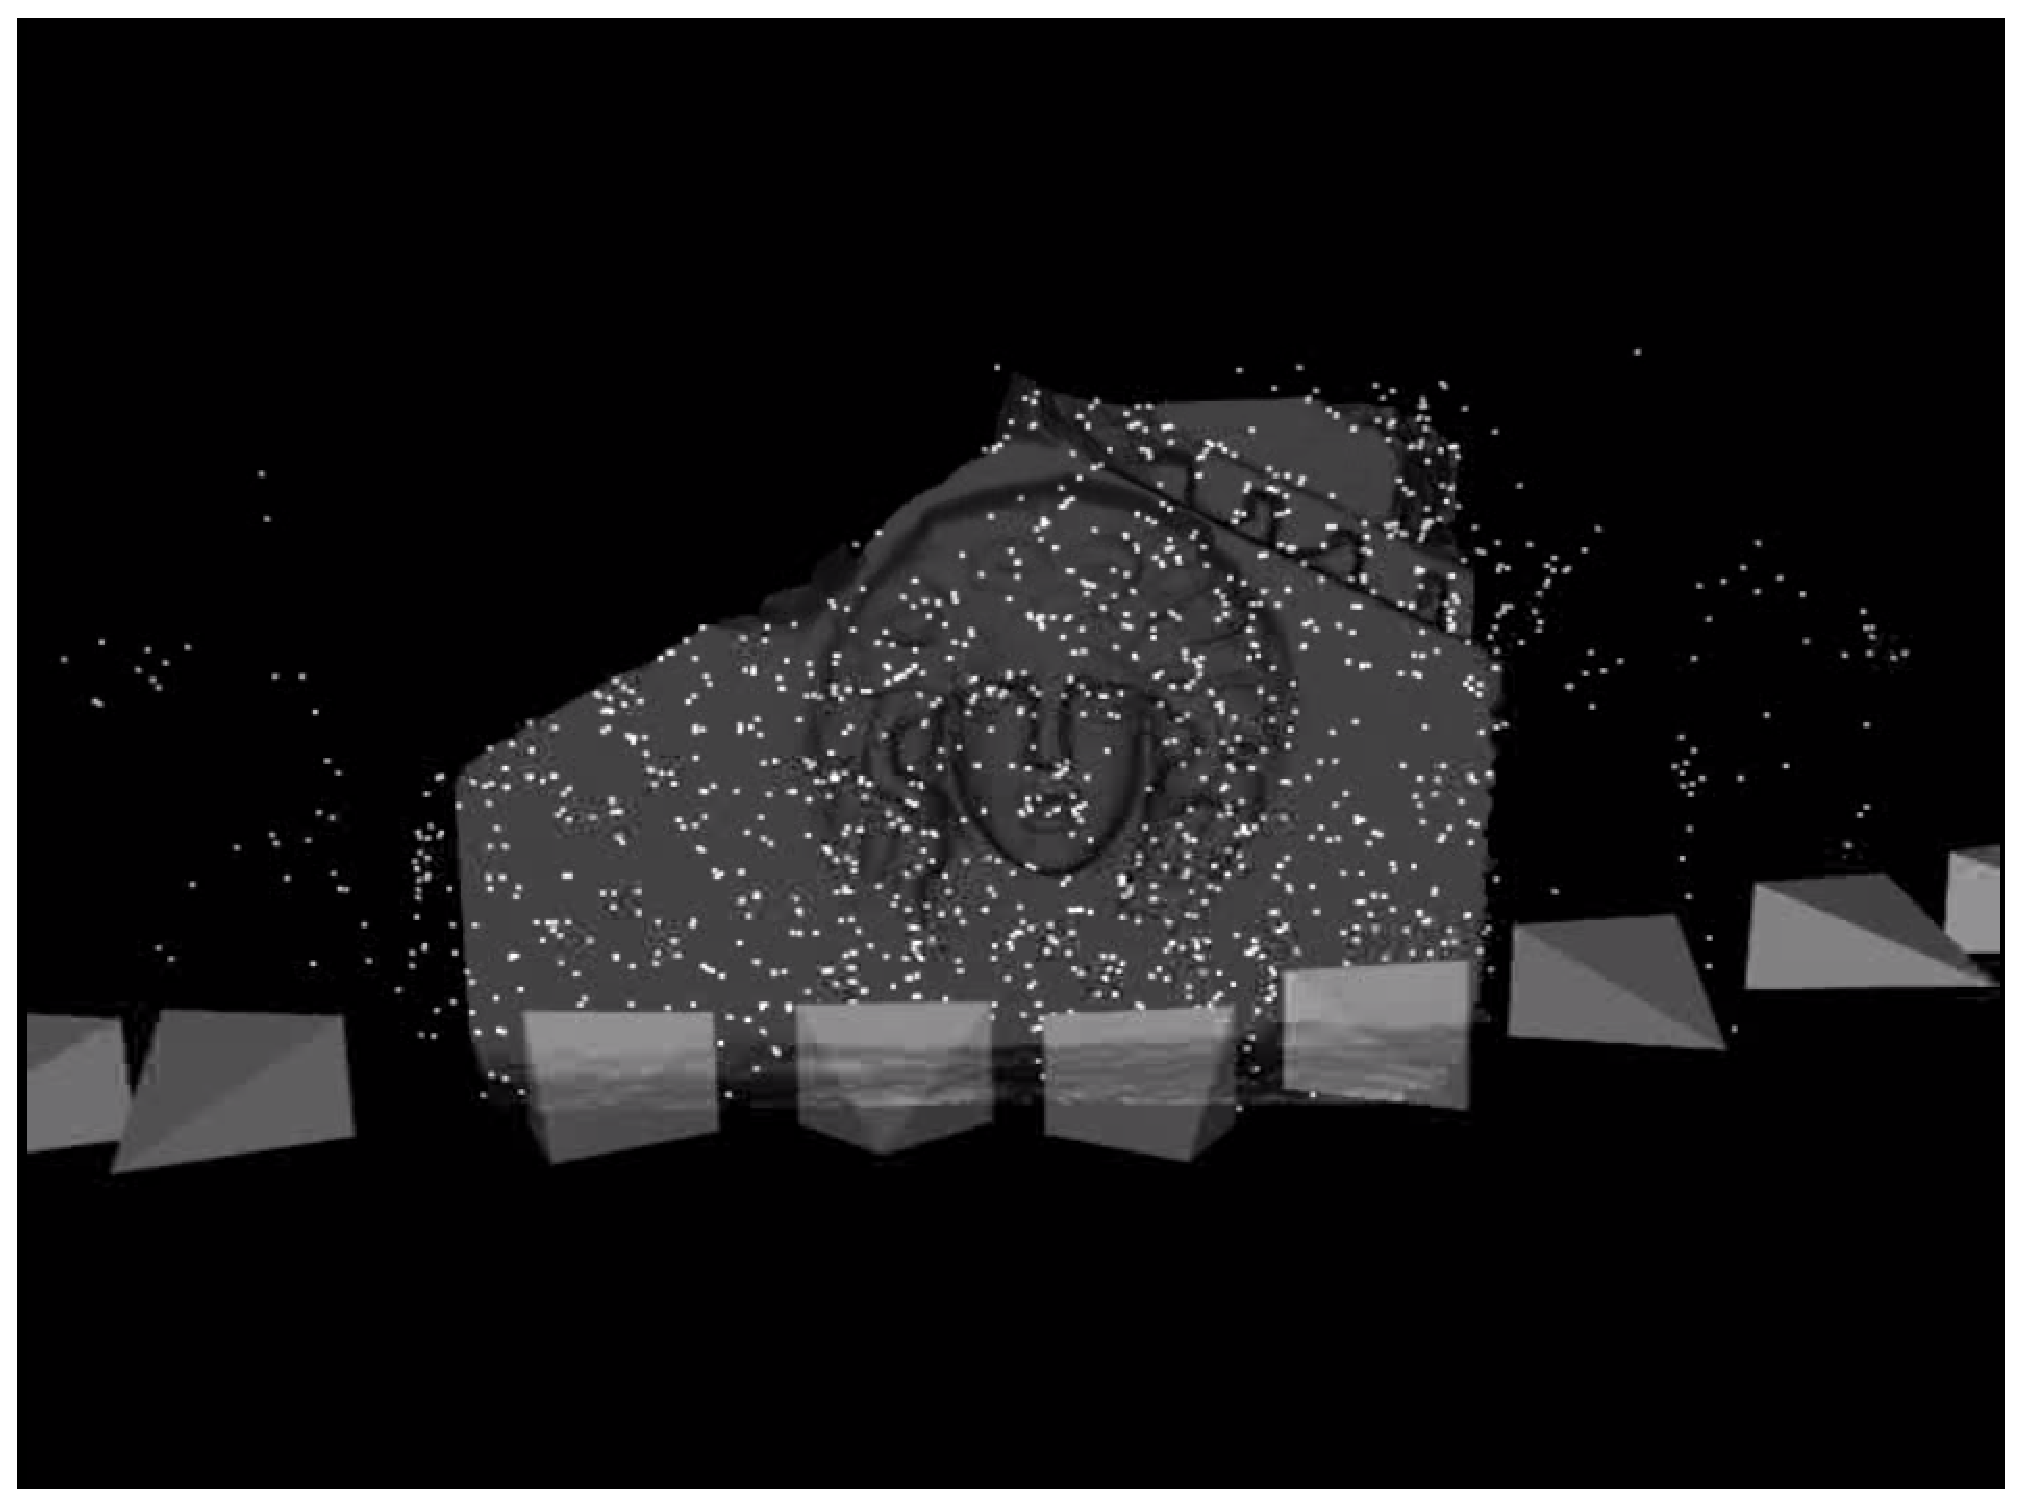
\includegraphics[scale=.2]{texturizacao1}}
\quad
\subfloat{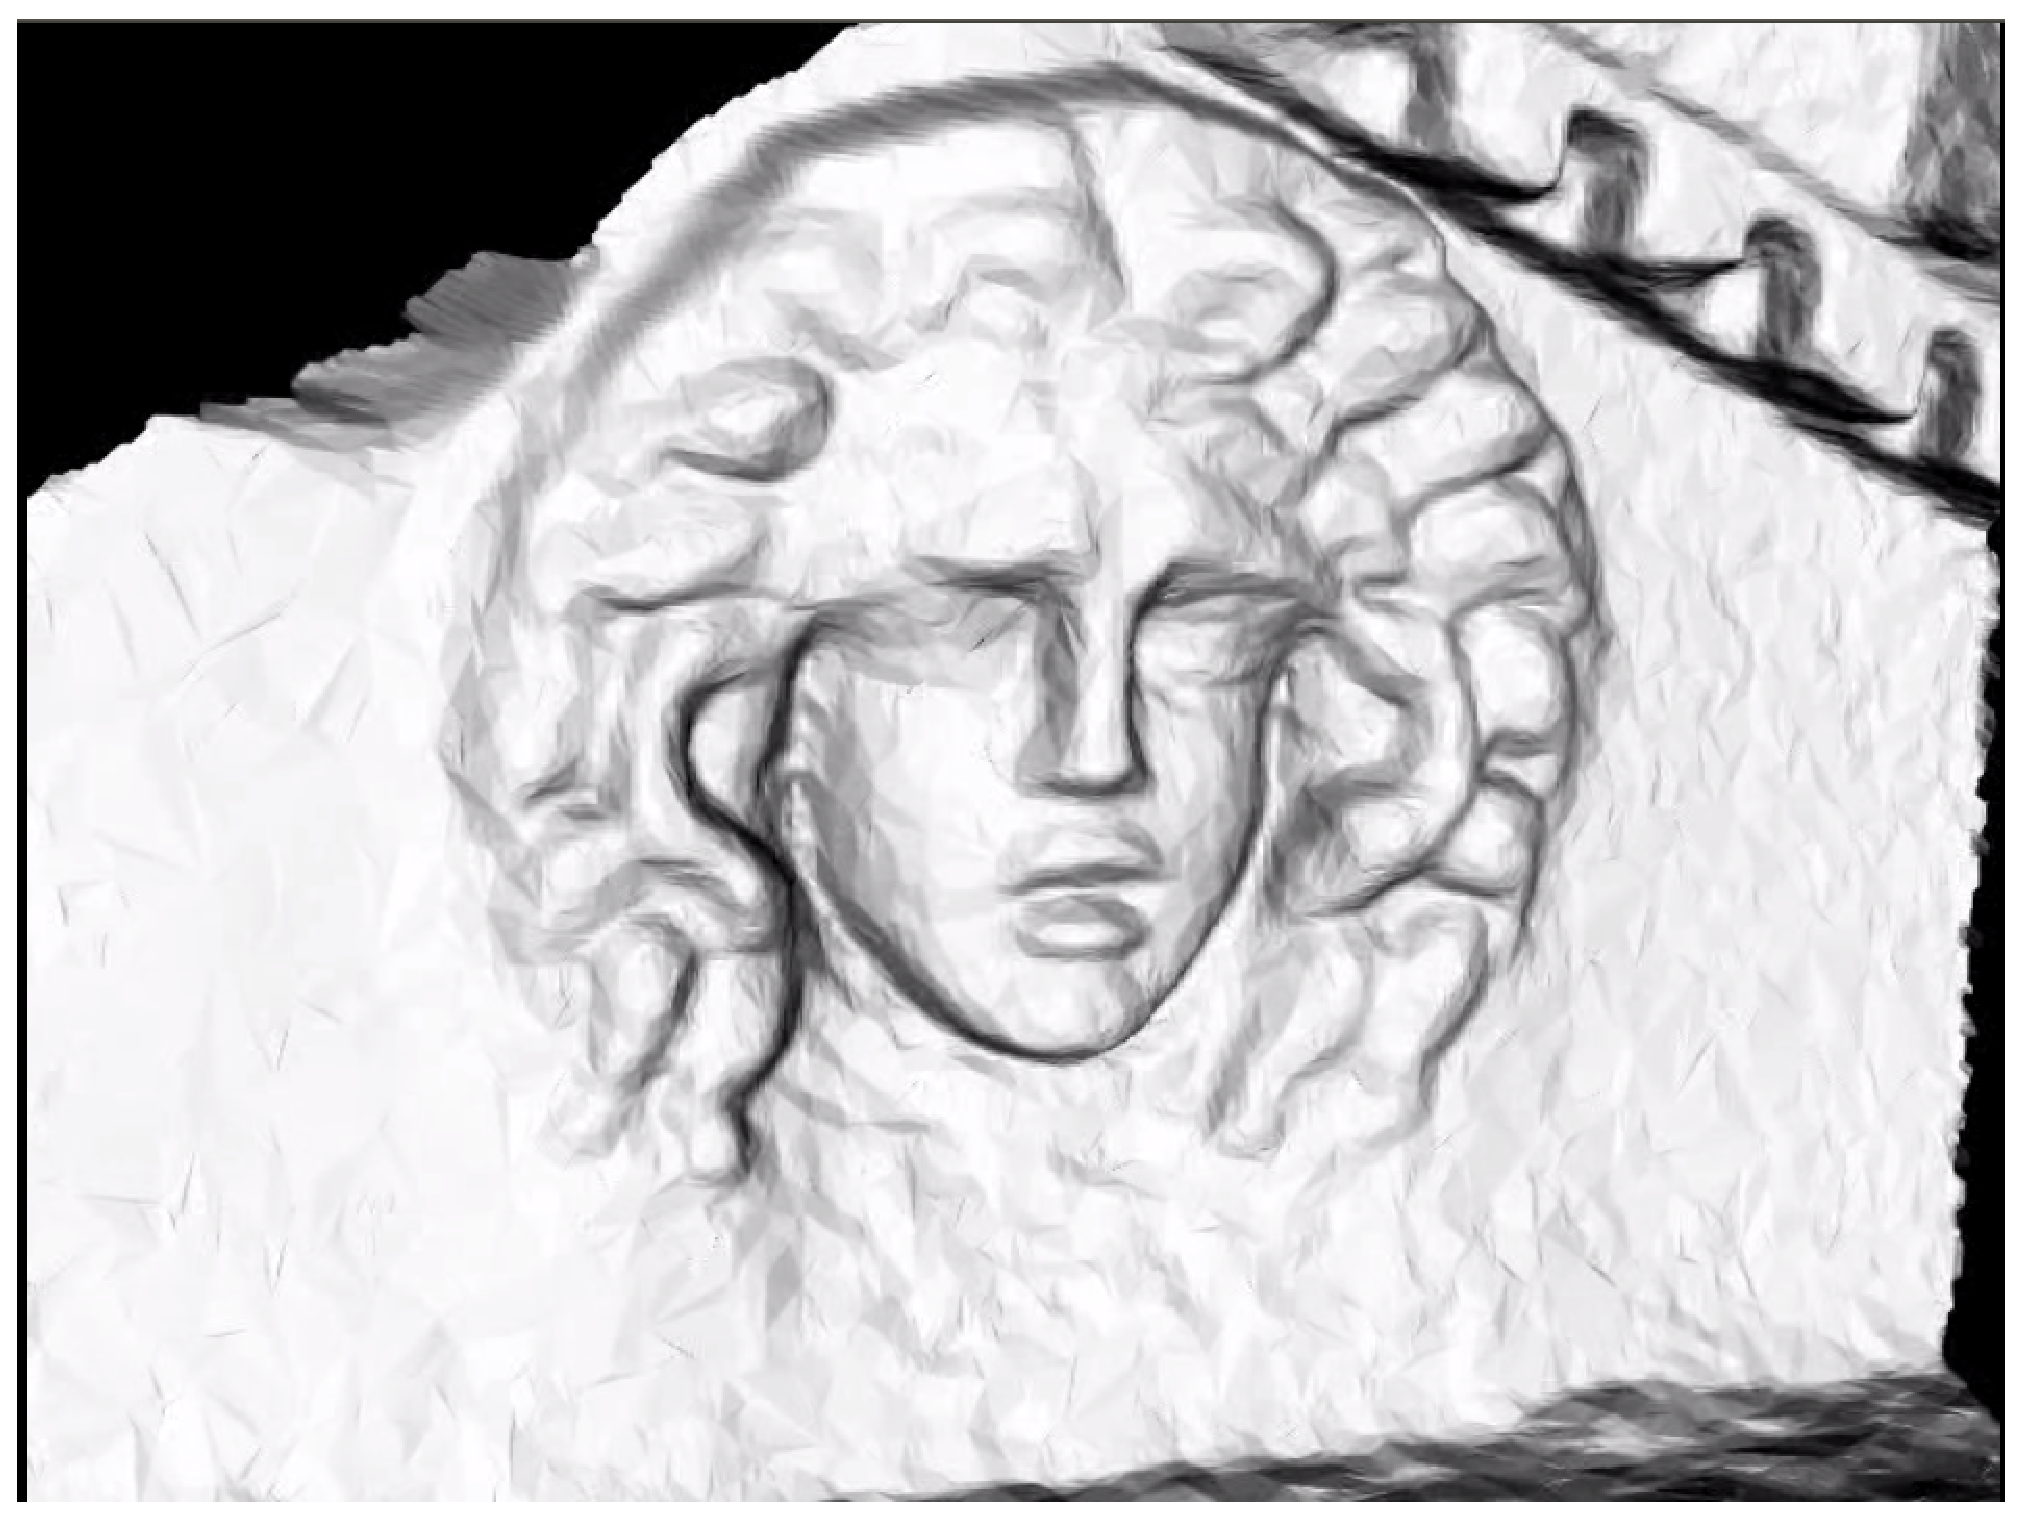
\includegraphics[scale=.2]{texturizacao2}}
\caption{{\it Em cima, duas imagens da medusa extraídas do vídeo. No meio, a nuvem de pontos obtida após a reconstrução 3D juntamente com as posições da câmera durante a confecção do vídeo. Em baixo, aplicação de interpolação de pontos e texturização.}}
\label{fig.medusa}
\end{figure}

\subsection*{Visão Geral}

A seção \ref{sec.geo-1-2-cam} engloba a teoria básica de geometria projetiva utilizada em visão computacional, com abordagens em termos de álgebra linear e usando o tipo de notação mais difundido entre pesquisadores da área. Além dos conceitos básicos, também são apresentados alguns conceitos e definições um pouco mais avançados indispensáveis ao entendimento das demais seções da dissertação, tudo com a finalidade de facilitar a compreensão do leitor sem a necessidade de consulta em outras publicações. Em seguida, há a apresentação da geometria epipolar, num sistema de visão estéreo com duas câmeras, bem como extração da matriz fundamental e a reconstrução das câmeras, usando essa abordagem bifocal que é mais comum do que a abordagem trifocal.

Na seção \ref{sec.astrom} temos o detalhamento de um artigo para a reconstrução de uma câmera a partir de objetos geométricos em 3D e suas respectivas imagens em 2D. A importância dessa publicação se verifica na utilização do Quatérnion de Hamilton para a parametrização da matriz de rotação da câmera, pois desta forma a matriz que possui nove componentes é parametrizada com apenas três variáveis. Outra vantagem é utilização das Bases de Gr\"obner e da Matriz de Ação para solução de sistemas de equações polinomiais de grau elevado e com muitas variáveis.

A geometria trifocal e suas características são abordadas na seção \ref{sec.geo-tri}, juntamente com a descrição dos benefícios do uso dessa geometria num sistema com três câmeras em comparação com uso da geometria epipolar nesse mesmo sistema. Após as comparações são apresentados métodos para a extração das matrizes fundamentais e métodos de reconstrução das câmeras a partir do tensor trifocal.  

Na seção \ref{sec.nister} há o detalhamento matemático da abordagem mais eficiente, até o momento, para a reconstrução 3D das câmeras num sistema trifocal. O artigo é bastante denso, com 25 teoremas, e apresenta a reconstrução de duas câmeras num sistema bifocal utilizando uma intrincada rede de conhecimentos de geometria projetiva. Depois da reconstrução das duas primeiras câmeras, é utilizado a reconstrução 3D de pontos para a reconstrução da terceira câmera, num procedimento similar ao apresentado na seção \ref{sec.astrom}, ou seja, os dois artigos quase se complementam. Esse trabalho deixa bem clara a dificuldade de se realizar a reconstrução num sistema com três imagens de quatro pontos 3D numa cena.

No apêndice \ref{sec.Apen-A} são fornecidas ferramentas de álgebra linear acompanhadas de algumas definições mais restritas à assimilação da dissertação. No apêndice \ref{sec.geo-algebrica} há uma breve introdução aos conceitos básicos de geometria algébrica seguidos da apresentação (informal e em termos de exemplos) de uma teoria para resolução de sistemas de equações polinomiais com várias variáveis.

